\documentclass[aspectratio=169]{beamer}
%\usepackage[english,greek]{babel}
%\usepackage[iso-8859-7]{inputenc}
\usepackage{euler}
\usepackage{graphicx,pgfplots,tikz}

\beamertemplatenavigationsymbolsempty

\begin{document}
	\begin{frame}{$c=1$}
		\begin{figure}
			\resizebox{\linewidth}{!}{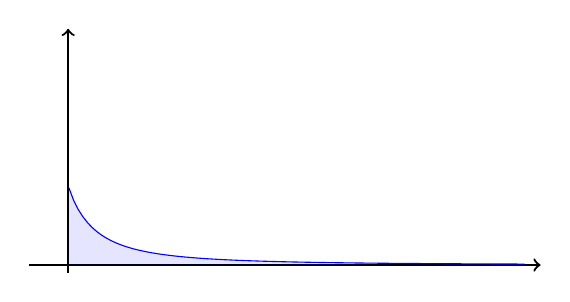
\begin{tikzpicture}
			\draw[thick,->] (-.5,0) -- (6,0);
			\draw[thick,->] (0,-.1) -- (0,3);
			\draw[blue, domain={0.01}:{5.8}, samples=100] plot (\x,{(1/(1+\x)-(1/(1+2*\x)))/\x});
			\draw[draw=none, fill=blue, fill opacity=.1, domain={0.01}:{5.8}, samples=100] plot (\x,{(1/(1+\x)-(1/(1+2*\x)))/\x}) -- (5.8,0) -- (0,0) -- cycle;
			\end{tikzpicture}}
		\end{figure}
	\end{frame}

\begin{frame}{$c=2$}
	\begin{figure}
		\resizebox{\linewidth}{!}{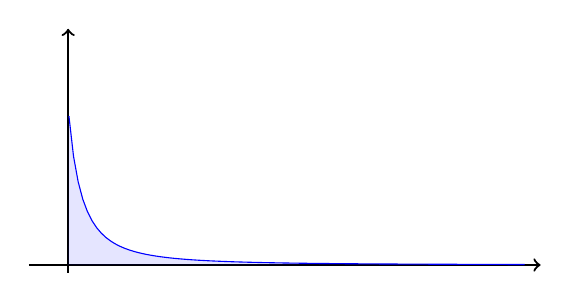
\begin{tikzpicture}
			\draw[thick,->] (-.5,0) -- (6,0);
			\draw[thick,->] (0,-.1) -- (0,3);
			\draw[blue, domain={0.01}:{5.8}, samples=100] plot (\x,{(1/(1+2*\x)-(1/(1+2*2*\x)))/\x});
			\draw[draw=none, fill=blue, fill opacity=.1, domain={0.01}:{5.8}, samples=100] plot (\x,{(1/(1+2*\x)-(1/(1+2*2*\x)))/\x}) -- (5.8,0) -- (0,0) -- cycle;
			\end{tikzpicture}}
	\end{figure}
\end{frame}

\begin{frame}{$c=3$}
	\begin{figure}
		\resizebox{\linewidth}{!}{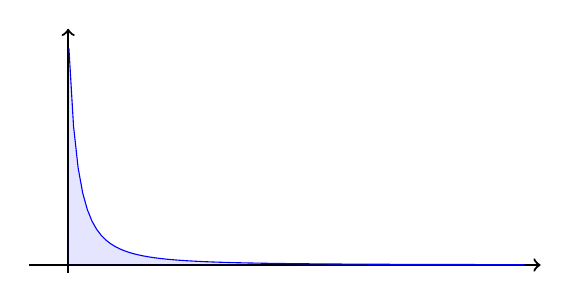
\begin{tikzpicture}
			\draw[thick,->] (-.5,0) -- (6,0);
			\draw[thick,->] (0,-.1) -- (0,3);
			\draw[blue, domain={0.01}:{5.8}, samples=100] plot (\x,{(1/(1+3*\x)-(1/(1+3*2*\x)))/\x});
			\draw[draw=none, fill=blue, fill opacity=.1, domain={0.01}:{5.8}, samples=100] plot (\x,{(1/(1+3*\x)-(1/(1+3*2*\x)))/\x}) -- (5.8,0) -- (0,0) -- cycle;
			\end{tikzpicture}}
	\end{figure}
\end{frame}
\begin{frame}{$c=4$}
	\begin{figure}
		\resizebox{\linewidth}{!}{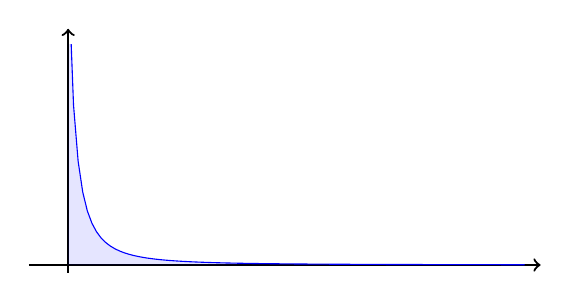
\begin{tikzpicture}
			\draw[thick,->] (-.5,0) -- (6,0);
			\draw[thick,->] (0,-.1) -- (0,3);
			\begin{scope}
			\clip (-.5,-.1) rectangle (6,2.8);
			\draw[blue, domain={0.01}:{5.8}, samples=100] plot (\x,{(1/(1+4*\x)-(1/(1+4*2*\x)))/\x});
			\draw[draw=none, fill=blue, fill opacity=.1, domain={0.01}:{5.8}, samples=100] plot (\x,{(1/(1+4*\x)-(1/(1+4*2*\x)))/\x}) -- (5.8,0) -- (0,0) -- cycle;
			\end{scope}
			\end{tikzpicture}}
	\end{figure}
\end{frame}
\begin{frame}{$c=5$}
	\begin{figure}
		\resizebox{\linewidth}{!}{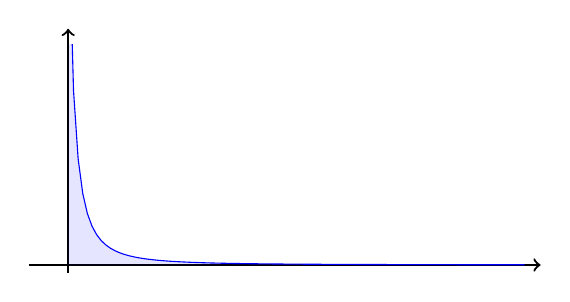
\begin{tikzpicture}
			\draw[thick,->] (-.5,0) -- (6,0);
			\draw[thick,->] (0,-.1) -- (0,3);
			\begin{scope}
			\clip (-.5,-.1) rectangle (6,2.8);
			\draw[blue, domain={0.01}:{5.8}, samples=100] plot (\x,{(1/(1+5*\x)-(1/(1+5*2*\x)))/\x});
			\draw[draw=none, fill=blue, fill opacity=.1, domain={0.01}:{5.8}, samples=100] plot (\x,{(1/(1+5*\x)-(1/(1+5*2*\x)))/\x}) -- (5.8,0) -- (0,0) -- cycle;
			\end{scope}
			\end{tikzpicture}}
	\end{figure}
\end{frame}
\begin{frame}{$c=6$}
	\begin{figure}
		\resizebox{\linewidth}{!}{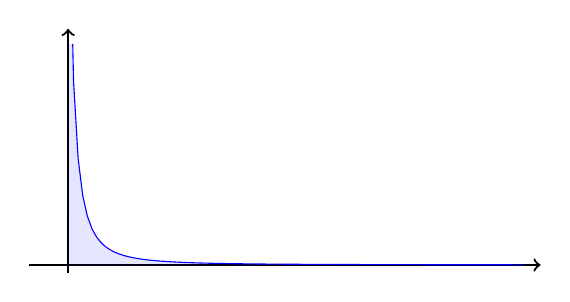
\begin{tikzpicture}
			\draw[thick,->] (-.5,0) -- (6,0);
			\draw[thick,->] (0,-.1) -- (0,3);
			\begin{scope}
			\clip (-.5,-.1) rectangle (6,2.8);
			\draw[blue, domain={0.01}:{5.8}, samples=100] plot (\x,{(1/(1+6*\x)-(1/(1+6*2*\x)))/\x});
			\draw[draw=none, fill=blue, fill opacity=.1, domain={0.01}:{5.8}, samples=100] plot (\x,{(1/(1+6*\x)-(1/(1+6*2*\x)))/\x}) -- (5.8,0) -- (0,0) -- cycle;
			\end{scope}
			\end{tikzpicture}}
	\end{figure}
\end{frame}

\begin{frame}{$c=7$}
	\begin{figure}
		\resizebox{\linewidth}{!}{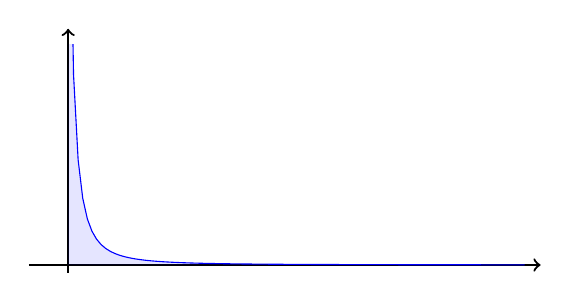
\begin{tikzpicture}
			\draw[thick,->] (-.5,0) -- (6,0);
			\draw[thick,->] (0,-.1) -- (0,3);
			\begin{scope}
			\clip (-.5,-.1) rectangle (6,2.8);
			\draw[blue, domain={0.01}:{5.8}, samples=100] plot (\x,{(1/(1+7*\x)-(1/(1+7*2*\x)))/\x});
			\draw[draw=none, fill=blue, fill opacity=.1, domain={0.01}:{5.8}, samples=100] plot (\x,{(1/(1+7*\x)-(1/(1+7*2*\x)))/\x}) -- (5.8,0) -- (0,0) -- cycle;
			\end{scope}
			\end{tikzpicture}}
	\end{figure}
\end{frame}
\end{document}